%!TEX TS-program = xelatex
%!TEX encoding = UTF-8 Unicode

\documentclass[12pt,a4paper,oneside]{report}
\usepackage{ntou-thesis}  % 已內含：fontspec, xeCJK, indentfirst, graphicx, hyperref 等
\usepackage{eso-pic}
\usepackage{graphicx}
\usepackage{color}
\usepackage{amssymb}    % \square for questionnaire checkboxes

%% ── 額外套件（ntou-thesis.sty 未載入者）──────────────────────────────────
\usepackage{rotating}    % sidewaystable / sidewaysfigure
\usepackage{multirow}    % 表格合併列
\usepackage{tabularx}    % 自動欄寬表格
\usepackage{pdfpages}    % \includepdf（書背用）
\usepackage{enumitem} % 用於精準控制條列式（研究目的）的間距
\usepackage{tikz}     % 【關鍵優化】用於直接在 LaTeX 內繪製高畫質流程圖
\usetikzlibrary{shapes.geometric, arrows.meta, positioning, calc}

\usepackage{silence}
\WarningFilter{latex}{Text page}
\usepackage{pgfplots}
\pgfplotsset{compat=1.18}
\captionsetup[table]{labelsep=space} % 將表格編號與標題之間改成「一個半形空白」，去掉冒號

%% ── XeTeX 中文斷行設定 ───────────────────────────────────────────────────
\XeTeXlinebreaklocale "zh"
\XeTeXlinebreakskip = 0pt plus 1pt
\tracinglostchars=0      % 抑制字元遺失警告

%% ── 垂直 CJK（書背旋轉字型）────────────────────────────────────────────
%% 僅在書背使用；若改由獨立 bookspine.tex 處理可移除此段。
\newCJKfontfamily{\vCJKFamily}[%
  Vertical    = RotatedGlyphs,
  RawFeature  = vertical%
]{NotoSerifTC-Regular}
\def\vCJKShiftSymbol#1{\raise.35em\hbox{#1}}
\def\vCJKBL{%
  \let\CJKsymbol\vCJKShiftSymbol
  \let\CJKpunctsymbol\vCJKShiftSymbol
}
\def\vCJK#1{\vCJKBL\vCJKFamily\rotatebox{270}{#1}}

%% ── 論文元資料（所有欄位集中於此）──────────────────────────────────────
\NTOUSetup{
  mainfont      = {Times New Roman},
  department    = {航運管理學系},
  departmenten  = {Shipping and Transportation Management},
  collegeen     = {College of Maritime Science and Management},
  degreezh      = {碩士},
  degreeen      = {Master of Business Administration},
  titlezh       = {你的題目},
  titleen = {\textmd{A Study on the Structural Relationships among Green Consumption Cognition, Attitude, and Behavior of Generation Z Consumers in Keelung City}},
  studentzh     = {你的姓名},
  studenten     = {Your Name},
  advisorzh     = {指導教授姓名~博士},
  advisoren     = {Name of Your Advisor},
  rocdate       = {中華民國 X 年 Y 月},
  endate        = {X},
  spineyear     = {X},
  logofile      = {ntou-logo.pdf}
}

\AtBeginDocument{%
  \setlength{\parskip}{1\baselineskip}%
}
\setcounter{secnumdepth}{3}

\begin{document}

%% ── 封面 ────────────────────────────────────────────────────────────────
\makeNTOUCover

%% ── 書背（獨立 PDF，由 bookspine.tex 編譯後匯入）────────────────────────
\clearpage
\thispagestyle{empty}
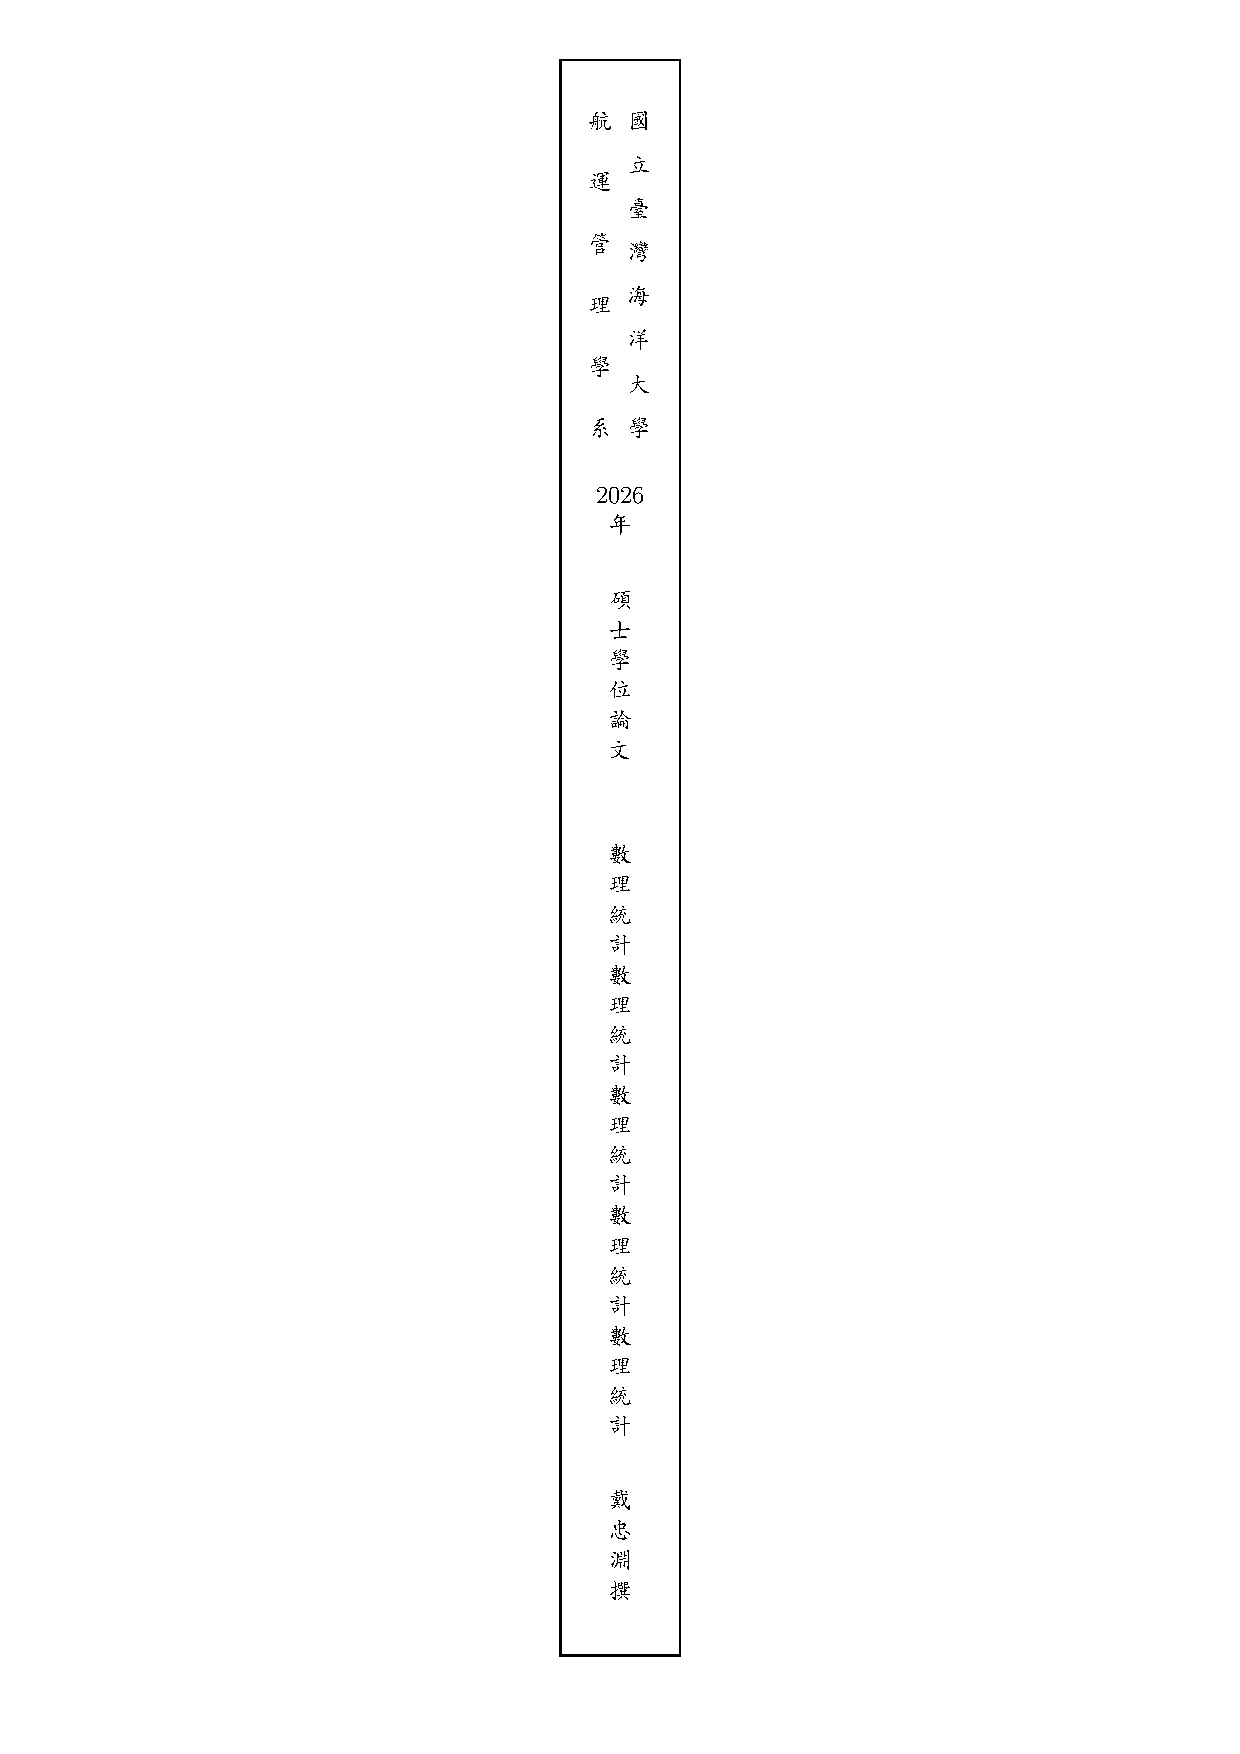
\includepdf{bookspine.pdf}
\clearpage

%% ── 書名頁 ──────────────────────────────────────────────────────────────
% --- 在想要加浮水印的該頁開頭插入以下程式碼 ---
% --- 在想要加浮水印的該頁開頭插入以下程式碼 ---
\AddToShipoutPicture*{
  \AtPageCenter{
    \makebox[0pt]{
      % 使用 \raisebox 將圖片向下偏移自身高度的一半，達成完美的垂直置中
      \raisebox{-0.5\height}{
        % opacity=0.1 代表透明度 10%（需要配合 graphicx 支援，或者圖片本身就是淡色）
        % 如果圖片太深，建議先用影像軟體將校徽透明度調淡
        
\includegraphics[width=0.9\textwidth]{Watermark_JPG.jpg}
      }
    }
  }
}
% ---------------------------------------------
% ---------------------------------------------
\makeNTOUTitlePage

%% ── 學位考試及格證明書 ──────────────────────────────────────────────────
%\makeNTOUCertificate

%% ── 前頁（Roman 頁碼）──────────────────────────────────────────────────
\NTOUFrontMatter


\begin{NTOUAcknowledge}
\thispagestyle{empty}
首先我要感謝我的指導老師對論文提出了許多寶貴意見，如果不是他，這篇論文可能早就寫完了。
同時也感謝我自己，為了能夠畢業，都一把年紀了這麼努力熬夜寫程式。如果你不逼自己一把，永遠不知道自己有多牛。
\end{NTOUAcknowledge}


\begin{NTOUAbstractZH}
\setcounter{page}{1} 

摘要

\vspace{-12pt}
\noindent \NTOUKeywordsZH{綠色消費認知、綠色消費態度、綠色消費行為}
\end{NTOUAbstractZH}

\begin{NTOUAbstractEN}

Abstract

\vspace{-12pt}
\noindent\NTOUKeywordsEN{Green Consumption Cognition, Green Consumption Attitude, Green Consumption Behavior}
\end{NTOUAbstractEN}

%\usepackage{zhnumber} % 用於將阿拉伯數字轉為中文（一、二、三）
%\usepackage{titletoc} % 用於自訂目錄格式

% 設定 Chapter 在目錄中的顯示格式
\titlecontents{chapter}[0em]
  {\addvspace{1em}\bfseries} % 目錄中的字體格式（粗體、加一點行距）
  {第{\thecontentslabel}章\quad} % 標籤格式：將 1 轉為 第一章
  {} % 無標籤時的格式
  {\titlerule*[0.7em]{.}\contentspage} % 引導線與頁碼

% ==================== 目錄與表次區 ====================
\clearpage
\begin{spacing}{1.0}
    
    % 1. 基本段距歸零
    \setlength{\parskip}{0pt}
    \setlength{\itemsep}{0pt}

    % 2. 強制歸零 tocloft 樣板在「章、節、圖、表」之間預設的垂直間距
    \setlength{\cftbeforechapskip}{0pt}
    \setlength{\cftbeforesecskip}{0pt}
    \setlength{\cftbeforetabskip}{0pt}
    \setlength{\cftbeforefigskip}{0pt}

    % 3. 攔截並封鎖底層偷偷加上的 \addvspace 間距
    \makeatletter
    \def\addvspace#1{}
    \makeatother

    % 產生目錄
    \phantomsection
    \addcontentsline{toc}{chapter}{目錄}
    \tableofcontents

    \clearpage
    
    % 產生表次
    \phantomsection
    \addcontentsline{toc}{chapter}{表次}
    \listoftables

    \clearpage
    
    % 產生圖次
    \phantomsection
    \addcontentsline{toc}{chapter}{圖次}
    \listoffigures

\end{spacing}
\clearpage
% ======================================================

\setlength{\parskip}{12pt}
\setlength{\itemsep}{12pt}

%% ── 正文（Arabic 頁碼）─────────────────────────────────────────────────
\NTOUMainMatter



\chapter{緒論}
 

\end{document}
